\section{Theoretical Background}
\label{sec:theory}

\subsection{Backpropagation Network}
Backpropagation networks are multi-layer feed-forward networks with supervised learning. There is no interconnection between neurons in the same layer but layers are fully connected to the next neighbouring layer in order to be able to do forward and backward propagation of values.

\subsubsection{Forward-propagation}
Each neuron in all layers but input layer disposes of a weight for each input initialized to a random value in range $<0,1>$, linear base function and sigmoidal activation function.

When forward propagating an input vector the vector is laid out onto the input neurons and the vector is recalculated using following formulas for the next layer until the input vector is propagated to the output layer which outputs the response of the whole network itself.

The base function is shown in equation \ref{eq:base}:

\begin{equation}
    f(\vec{x}) =\sum_{i = 0}^{n} w_i x_i
    \label{eq:base}
%    f(u) = \frac{1}{1 + e^{-\lambda u}}
\end{equation}

where $ \vec{x} $ is the input vector, $ w $ are weights for each input of given neuron and $ n $ is the length of the neuron input vector and bias (term used as in \cite{deeplearning}\cite{elements}) value resulting in $ n = |x| + 1$.

The sigmoidal activation function is presented in equation \ref{eq:act} where $ \lambda $ is a constant set to $ \lambda = 1 $ and in further equations left out because of this fact.

\begin{equation}
    g(u) = \frac{1}{1 + e^{-\lambda u}}
    \label{eq:act}
\end{equation}

The output of a neuron is then given by using the equations \ref{eq:base} and \ref{eq:act}:

\begin{equation}
    y = g( f( \vec{x} ) )
    \label{eq:output}
\end{equation}


\subsubsection{Back-propagation}
Back-propagation is used only when one trains the network and is one of the base methods for training feed-forward networks. The method is based on adjusting weights depending on the error calculated by equation \ref{eq:err} for an output neuron $ p $ using produced output ($ o $) and desired output ($ d $) values.

\begin{equation}
    E_p = \frac{1}{2} \sum_{j = 1}^{m} (d_{pj} - o_{pj})^2
    \label{eq:err}
\end{equation}

The change of weights is calculated using equation \ref{eq:delta} where $ \nabla E_p $ is the derived error gradient and $ \mu $ the learning rate.

\begin{equation}
    \Delta \vec{w_p} = -\mu \nabla E_p
    \label{eq:delta}
\end{equation}

To calculate one particular change of weight we use formula \ref{eq:neuron-delta} where $ l $ is the given layer of the network, $ j $ is the $j$-th neuron in layer $ L $ and $ i $ is the $i$-th input of the neuron $ j $.

\begin{equation}
    \Delta {^lw}_{ji} = \mu {^l\delta}_j {^lx}_i
    \label{eq:neuron-delta}
\end{equation}

For the output layer $ l $ of the network we use formula \ref{eq:output-err}.

\begin{equation}
    \delta_j^L = (d_j - {^ly}_j) {^ly}_j(1 - {^ly}_j)
    \label{eq:output-err}
\end{equation}

For hidden layers of the network, we use the same principle propagating the error backwards from the output layer as shown in equation \ref{eq:prop-err} where $\lambda = 1$ and therefore left out.

\begin{equation}
    \Delta {^l w}_{ji} = \mu {^l\delta}_j {^lx}_i = \mu \sum_{k = 1}^{n_{l+1}} (^{l+1}\delta_k {^{l+1}w}_{kj}) {^ly}_j (1 - ^ly_j){^lx}_i
    \label{eq:prop-err}
\end{equation}

Each repetition of forward and backward propagation of all inputs is called an epoch. Finally, we can choose when to update the weights, in batches after all input vectors were processed or using the stochastic method where weights are updated after processing each input vector.

\subsection{Examon}
\label{sec:examon}
Examon\cite{examon} framework is used for exascale monitoring of supercomputing facilities. It is built on top of MQTT protocol\cite{locke2010mqtt} which allows measured metrics to be sent to a central broker where received data are processed and stored in KairosDB\cite{KAIROS} database utilizing Cassandra\cite{CASSANDRA} cluster.

\begin{figure}[ht]
    \centering
    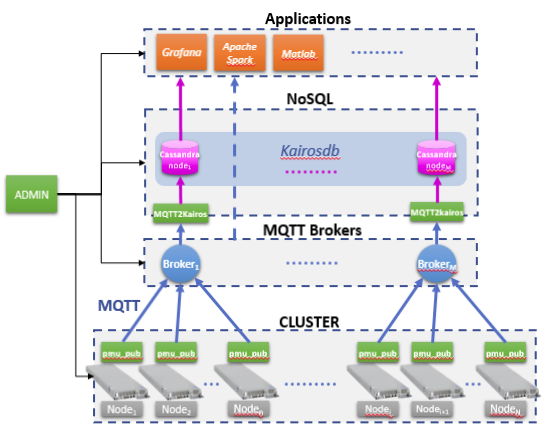
\includegraphics[width=0.45\linewidth]{examon-architecture}
    \caption{Examon framework architecture}
    \label{arch}
\end{figure}

KairosDB is used for storing metric data in time-series format whereas Cassandra, serving as a backend for KairosDB is also used for storing job-related data. More on data semantics is described~in~\ref{sec:data}.

